%!TEX root = thesis.tex

\documentclass[12pt]{article}
\usepackage[spanish]{babel}

% Margenes
\usepackage{geometry}
\geometry{
  letterpaper,
  top=4cm,
  bottom=3cm,
  left=4cm,
  right=3cm
}

% Fuente
\usepackage{fontspec}
\setmainfont{Times New Roman}
\usepackage{csquotes}

\renewcommand{\baselinestretch}{1.5}

\usepackage{graphicx}
\usepackage{amsmath}
\usepackage{hyperref}
\usepackage{float}
\usepackage{parskip}
\usepackage[spanish]{cleveref}

\usepackage{algorithm}
\usepackage{algpseudocode}

\usepackage[caption = true]{subfig}

\usepackage{natbib}
\bibliographystyle{apalike}

\begin{document}

\title{Análisis Descriptivo y Predictivo Basado en Datos del Tráfico Vehicular en Antofagasta: Un Enfoque a partir de Reportes de Conductores}
\author{Richard Peña Bonifaz}
\date{\today}
\maketitle

\section*{Dedicatoria}

A todas las personas que estuvieron conmigo y me alentaron en los momentos más difíciles.

\section*{Reconocimientos}

A los profesores apasionados por su trabajo, que no solo transmiten conocimiento, sino también la pasión por el saber y la aplicación de la materia que imparten.

\newpage
\tableofcontents
\newpage

\section*{Resumen}

El proyecto desarrollado tuvo como propósito la creación de una herramienta efectiva para analizar y predecir, con alta confiabilidad, el comportamiento del tráfico vehicular en la ciudad de Antofagasta, utilizando datos provenientes de la plataforma Waze Cities \citep{wazecities2024}. Esta plataforma, alimentada por su comunidad de usuarios, proporciona información en tiempo real que permite obtener una visión detallada de los eventos de tráfico en la ciudad. La investigación resultante generó información relevante para la gestión del tráfico, facilitando la toma de decisiones por parte de las autoridades locales, con miras a mejorar la seguridad vial y optimizar la eficiencia del flujo vehicular. A partir del análisis y explotación de estos datos, fue posible identificar patrones y tendencias que, al ser integrados en la planificación urbana, permiten optimizar rutas críticas, reducir la congestión y disminuir la probabilidad de accidentes.

Se consiguió obtener un modelo capas de predecir el comportamiento del tráfico con una precisión del 85.83\% y un F1-score de 88.23\%, de acuerdo con el análisis de bondad de ajuste realizado al modelo final, el cual fue entrenado utilizando el algoritmo de clasificación XGBoost. Se utilizaron alrededor de 64.708 eventos para el entrenamiento.

\section{Introducción}
\subsection{Descripción del problema}

Antofagasta, una ciudad con más de 106,000 vehículos en circulación \citep{comision2023}, enfrenta desafíos significativos en la gestión de su tráfico vehicular. Durante el año 2023, se registraron 1,715 accidentes, los cuales resultaron en 31 fallecidos y 102 heridos graves \citep{comision2023}. Tuvo un crecimiento de su parque automotriz de 0.8\% y 3.5\% en los años 2022 y 2023 respectivamente según datos del INE \citep{ine2023}.

La infraestructura vial limitada cuenta con dos arterias principales para poder atravesar la ciudad, la Avenida Edmundo Perez Zujovic y la Avenida Pedro Aguirre Cerda, La segunda solo presente en la mitad del recorrido, por lo que para la otra mitad, se deben utilizar diferentes alternativas en similares alturas de la ciudad, ninguna de estas continuas. Esto posiciona a la Avenida Edmundo Perez Zujovic, la cual en el sector sur de la ciudad se encuentra con Avenida Grecia y Avenida Ejército, como la única vía continua que atraviesa la ciudad completamente. Esta particularidad dada las características geográficas de Antofagasta sumada a la alta concentración de vehículos, genera una alta congestión y  riesgo de accidentes, especialmente en las zonas anteriormente mencionadas.

Actualmente, no existe algún sistema de monitoreo en tiempo real que permitan gestionar el tráfico de manera proactiva \citep{goodall2019}. Los sistemas de monitoreo tradicionales, como son la gestión de semáforos y el estudio de vías, es valioso para la administración del flujo vehicular y la estandarización de las intersecciones. Sin embargo, tiene limitaciones por ser estático para la vía en donde el diseño fue realizado. Este tipo de gestión tiene la limitación de no permitir una visión global del flujo vehicular, como también la poca flexibilidad ante los cambios que se generan en el entorno \citep{auld2009}.

Explorar nuevas fuentes de datos, como los eventos vehiculares en la ciudad, o la gestión a través de visión por computadora, son herramientas que permiten gestionar de forma eficiente y efectiva el flujo vehicular, proporcionando datos en tiempo real, también ofrecen opciones de automatización y predictibilidad \citep{chen2015}. Contar con grandes volúmenes de datos permite desarrollar modelos inteligentes para la gestión del tráfico vehicular.

Waze recopila datos de eventos reportados por los usuarios, los cuales cuentan con tres aspectos principales; el tiempo, la ubicación, y el tipo de evento. Esta categorización permite poder desarrollar modelos que detecten patrones y puedan estimar con alta probabilidad eventos futuros, basándose en los datos pasados. Esta opción entrega una visión global de la ciudad, para poder detectar focos de atención en cuanto a la ocurrencia de accidentes y la congestión vehicular. El uso de datos colaborativos, como los reportados por usuarios en Waze, ha demostrado ser una fuente válida para el análisis y predicción de patrones de tráfico urbano, permitiendo detectar focos críticos de congestión y accidentes \citep{ferreira2017waze}.

La plataforma Waze Cities, permite a ciudades poder obtener datos para gestionar el tráfico vehicular con herramientas inteligentes, esto conlleva a mejorar la seguridad y la eficiencia en el tráfico vehicular, usando una fuente de dato ya existente \citep{wazecitiescasestudies2024}.

\subsection{Objetivo general}

Realizar un análisis exhaustivo del comportamiento del tráfico en la ciudad de Antofagasta basado en los eventos reportados por los conductores en la plataforma Waze. El objetivo final es generar información relevante que contribuya a la gestión eficiente del tráfico, mejorando la seguridad vial y optimizando el flujo vehicular.

\subsection{Objetivos específicos}

\begin{itemize}
    \item Obtener datos suficientes y representativos sobre los eventos de tráfico en Antofagasta mediante la API de Waze Cities.
    \item Realizar un análisis descriptivo de los datos recolectados para identificar patrones y tendencias relevantes en el comportamiento del tráfico.
    \item Presentar información visualmente comprensible y útil para las autoridades de gestión vial, facilitando la implementación de políticas y acciones basadas en datos.
    \item Utilizar los datos disponibles para desarrollar modelos predictivos de tráfico que permitan anticipar eventos y tomar decisiones proactivas en la gestión vial.
\end{itemize}

\subsection{Alcances}

Los datos utilizados corresponden al periodo desde octubre de 2024 hasta abril de 2025, en el sector urbano de la ciudad de Antofagasta, desde la zona norte urbana actual, sector Costa Laguna, hasta la zona sur, salida a camino de la minería, excluyendo el camino a puerto Coloso.

El área de estudio está delimitada por las coordenadas geográficas 23.35°S a 23.65°S de latitud y 70.36°O a 70.45°O de longitud, correspondientes al sistema de referencia EPSG:4326 (WGS84).

\section{Marco teórico}

El tráfico vehicular en entornos urbanos presenta un comportamiento complejo e impredecible, lo que dificulta su gestión eficiente. No obstante, el avance de las tecnologías móviles y la popularidad de aplicaciones como Waze permiten disponer de datos en tiempo real generados por los propios usuarios. Este proyecto se apoya en técnicas de análisis de datos y aprendizaje de máquinas (Machine Learning) para convertir esta información en herramientas útiles para la gestión vial. La utilización de datos geoespaciales, junto con la automatización de los procesos de recolección, análisis y visualización, constituye una solución costo-efectiva para mejorar la planificación del tráfico \citep{barcelo2005}.

\subsection{Gestión de la seguridad vial}

Existen diferentes estrategias para la gestión vehicular, desde sistemas manuales como la dirección del tránsito por carabineros, o más automatizados, como la gestión inteligente de semáforos. En términos de seguridad, para evitar la ocurrencia de accidentes, podemos aplicar la jerarquía de control de riesgo \cref{fig:jerarquia_riesgos}. Esta busca abordar desde la medida de mayor impacto, hasta la de menor impacto en la exposición al riesgo. Se divide en dos grupos principales, las barreras duras y las barreras blandas (administrativas). El primer grupo consta de la eliminación del agente de riesgo, la sustitución por uno de menor exposición y medidas ingenieriles, que buscan administrar la exposición con algún rediseño u organización. Las medidas administrativas constan de diferentes estrategias que puedan cambiar el comportamiento, el cuidado o la visibilidad de la exposición, por último, los elementos de protección personal, que buscan mitigar el daño ante algún posible accidente \citep{niosh2024}.

\begin{figure}[h]
    \centering
    \includegraphics[width=0.8\textwidth]{images/jerarquia_control_riesgo.png}
    \caption{Jerarquía de control de riesgos. Fuente: \citet{niosh2024}.}
    \label{fig:jerarquia_riesgos}
\end{figure}

La eliminación de la necesidad de transporte, puede ser abordada con estrategias como el fomento del teletrabajo para los puestos que lo permitan, o formas en que las personas se encuentren más cerca de sus trabajos, eliminando la necesidad de transporte en vehículo. La sustitución se genera fomentando el uso de transporte público, el uso de medios alternativos de transporte, como las bicicletas o el uso compartido de vehículos. Las medidas de ingeniería buscan optimizar en cuanto a tránsito y en seguridad el flujo vehicular, puede ser el rediseño del plano urbano, el diseño de vehículos más seguros, monitoreo a través de radares, cámaras y GPS, planificación de rutas y nuevas vías de tránsito. Como medidas administrativas se encuentran la educación vial, la señalización y los límites de velocidad. En cuanto a elementos de protección personal, se posiciona el uso de cinturón de seguridad, la instalación de airbags, barreras anti-vuelco y barreras de contención en las vías.

\subsection{Ciencia de datos para el análisis de comportamiento}

Entender el comportamiento del tráfico vehicular, permite desarrollar medidas ingenieriles que disminuyan la probabilidad de accidentes, gestionando diversas variables como la congestión vehicular, los horarios con mayor probabilidad de accidentes y los sectores con mayor frecuencia de accidentes. La ciencia de datos permite, a través del uso de diferentes herramientas estadísticas, predecir con un grado de certeza conocido, la probabilidad de que ocurra un accidente tomando en cuenta variables que puedan ser determinantes para la ocurrencia de los mismos.

Usando datos de eventos pasados, es posible generar modelos que, a partir de una entrada, entreguen una salida determinada según ciertos parámetros, esto se conoce como análisis predictivo. El análisis predictivo consiste en entrenar modelos con datos históricos para anticipar resultados futuros, utilizando distintas técnicas de aprendizaje automático, las cuales pueden clasificarse en aprendizaje supervisado, no supervisado y por refuerzo \citep{murphy2012machine, geron2019hands, bishop2006pattern}.

En el aprendizaje supervisado, el modelo recibe tanto los datos de entrada como los de salida esperada, lo que le permite aprender patrones y realizar predicciones sobre nuevos datos con base en ese entrenamiento. El aprendizaje no supervisado utiliza datos de entrada, buscando estructuras o patrones en los mismos sin una clasificación específica, dejando la interpretación a cargo del especialista. Finalmente, en el aprendizaje por refuerzo, el modelo recibe una entrada, ejecuta una acción o predicción, y ajusta su comportamiento en función de una retroalimentación positiva o negativa, con el objetivo de maximizar el rendimiento a lo largo del tiempo.

Adicionalmente, los modelos pueden clasificarse según el tipo de salida que generan: modelos de regresión, que entregan valores numéricos continuos, y modelos de clasificación, que asignan las observaciones a una o más categorías previamente definidas. En estos últimos, el resultado se expresa como una distribución de probabilidades, y se considera como salida final la categoría con mayor probabilidad.

En este estudio se empleó un modelo supervisado de clasificación, con el objetivo de estimar la probabilidad de ocurrencia de un accidente, considerando dos posibles resultados: “ocurre” o “no ocurre”.

Para evaluar el rendimiento del modelo se utilizaron métricas ampliamente empleadas en problemas de clasificación binaria, tales como la exactitud (\textit{accuracy}), la precisión (\textit{precision}), la sensibilidad (\textit{recall}) y la medida F1 (\textit{F1-score}) \citep{manning2008}. La exactitud representa el porcentaje total de predicciones correctas sobre el total de casos evaluados. La precisión corresponde a la proporción de casos positivos correctamente identificados por el modelo, es decir, el número de verdaderos positivos dividido por el total de predicciones positivas. Por su parte, la sensibilidad —también conocida como \textit{recall}— mide la capacidad del modelo para identificar correctamente todos los casos positivos reales, dividiendo los verdaderos positivos por el total de casos positivos reales. La medida F1, en tanto, es la media armónica entre precisión y sensibilidad, y proporciona una visión equilibrada del desempeño del modelo cuando es necesario considerar tanto los errores por omisión como los errores por comisión.

Además, se construyó una matriz de confusión, la cual permite observar el número de aciertos y errores cometidos en cada clase —“ocurre” y “no ocurre”— lo que facilita una evaluación más detallada del comportamiento del modelo. Este análisis es clave para comprender sus limitaciones y fortalezas, especialmente en aplicaciones reales relacionadas con la predicción de accidentes de tránsito.

Las fórmulas utilizadas para el cálculo de estas métricas son las siguientes:

\[
\begin{aligned}
\text{Exactitud (Accuracy)} &= \frac{TP + TN}{TP + TN + FP + FN} \\
\text{Precisión (Precision)} &= \frac{TP}{TP + FP} \\
\text{Sensibilidad (Recall)} &= \frac{TP}{TP + FN} \\
\text{Medida F1 (F1-score)} &= 2 \cdot \frac{\text{Precisión} \cdot \text{Sensibilidad}}{\text{Precisión} + \text{Sensibilidad}}
\end{aligned}
\]

donde \( TP \) son los verdaderos positivos, \( TN \) los verdaderos negativos, \( FP \) los falsos positivos y \( FN \) los falsos negativos.


\subsection{Análisis geoespacial}

Waze entrega las coordenadas geoespaciales de los eventos de tráfico en el sistema de referencia \textbf{EPSG:4326}. Este sistema corresponde al datum geodésico global \textbf{WGS84 (World Geodetic System 1984)}, ampliamente utilizado en aplicaciones de posicionamiento global (GPS) y cartografía digital \citep{epsg4326, wgs84_nima}. En EPSG:4326, las coordenadas están expresadas en grados decimales de latitud y longitud, lo cual es adecuado para visualización, pero no para realizar cálculos métricos directos como distancias o áreas.

Para llevar a cabo análisis espaciales cuantitativos sobre los eventos reportados por Waze —incluyendo cálculos de distancia, densidad y agrupación geográfica— fue necesario transformar dichas coordenadas a un sistema proyectado con unidades métricas.

La transformación se realizó utilizando la proyección Transversa de Mercator (Transverse Mercator), en su implementación como zona UTM 19 Sur (EPSG:32719). Esta proyección es conforme y está basada en el elipsoide WGS84, con un meridiano central en $\lambda_0 = -69^\circ$, un factor de escala $k_0 = 0.9996$, y un falso este de $500\,000$ m. Para el hemisferio sur, además, se aplica una corrección vertical de $10\,000\,000$ m a la coordenada norte. Esto se detalla en el Apéndice~\ref{ap:utm}.

Esta transformación se aplicó mediante la función \texttt{to\_crs} de la librería \texttt{GeoPandas}, la cual utiliza internamente la librería \texttt{Pyproj} como interfaz con la librería PROJ \citep{gdal_proj, pyproj, geopandas}.

La elección de EPSG:32719 permite minimizar la distorsión local, ya que el sistema UTM divide el globo en zonas longitudinales estrechas, optimizando la precisión en cada región. Al ser una proyección conforme y métrica, asegura que las distancias, áreas y densidades calculadas sobre el plano proyectado sean válidas y consistentes con el Sistema Internacional de Unidades \citep{epsg32719}.

\subsection{Aprendizaje automático}

A medida que la cantidad de datos aumenta, el modelo requiere ser reentrenado para incorporar los nuevos registros y así actualizar sus parámetros. Este proceso de aprendizaje continuo permite que el modelo se adapte a las variaciones que puedan presentarse en los patrones de tráfico vehicular a lo largo del tiempo. Para asegurar esta adaptabilidad, se programó una frecuencia de reentrenamiento mensual, lo que implica la incorporación de aproximadamente 9.244 nuevos datos al modelo cada mes. El reentrenamiento periódico resulta fundamental para mantener la vigencia y precisión del modelo, ya que permite integrar las tendencias más recientes y responder oportunamente a los cambios en las condiciones del tráfico \citep{gama2014concept}.


Para la gestión de los modelos se utilizó \texttt{MLFlow}, un \texttt{framework} que permite gestionar las versiones de los modelos y almacenarlos en una base de datos, asegurando la persistencia de los mismos. También permite almacenar las diferentes métricas de cada versión del modelo \citep{mlflow2025}.

Para la gestión del modelo, en cuanto a su implementación, mantenimiento y actualización, se programó con \texttt{APSCheduler}, una librería de tareas asíncronas en Python \citep{apscheduler2025}.

\subsection{Investigaciones previas}

El análisis del tráfico vehicular y la predicción de accidentes han sido objeto de múltiples estudios en los últimos años. Por ejemplo, \citet{barcelo2005} exploraron simulaciones dinámicas de redes de tráfico utilizando AIMSUN, destacando su capacidad para modelar escenarios urbanos complejos. Por otro lado, \citet{vanlint2005} desarrollaron modelos basados en redes neuronales para predecir tiempos de viaje en autopistas, incluso en condiciones de datos faltantes, demostrando la utilidad de enfoques basados en aprendizaje automático.

En el ámbito de la gestión de tráfico basada en datos, \citet{chen2015} propusieron enfoques impulsados por datos para la predicción y gestión del tráfico, enfatizando la importancia de integrar fuentes de datos en tiempo real. Asimismo, \citet{goedertier2009robust} introdujeron técnicas para descubrir procesos robustos mediante eventos negativos artificiales, lo que permite abordar problemas de clasificación supervisada en contextos de tráfico.

Más recientemente, \citet{berhanu2024} aplicaron aprendizaje automático y análisis espacial para predecir accidentes de tráfico y optimizar rutas en redes urbanas congestionadas, destacando la relevancia de combinar modelos predictivos con análisis geoespacial.

\subsection{Metodología}

Se realiza un análisis geoespacial con el objetivo de identificar puntos críticos, como vías principales, calles secundarias y zonas de alto tráfico. Este análisis se llevó a cabo utilizando \texttt{GeoPandas}. Además, se analizan series temporales para detectar patrones y tendencias del tráfico, identificando estacionalidades en el comportamiento. Los resultados se presentan mediante técnicas de visualización que permitien interpretar las tendencias y puntos de interés de manera efectiva.

El pipeline de datos incluye una base de datos relacional para almacenar los datos, un flujo ETL (Extract, Transform, Load) para procesarlos y un servidor web para visualizarlos. Se utilizó PostgreSQL \citep{postgres2025} como base de datos, Memcached  \citep{memcached2025} como base de datos de caché, APScheduler para la programación de tareas y Dash \citep{dash2025} como herramienta de visualización. Este enfoque permitió automatizar el flujo de datos y garantizar la actualización constante de la información.

Adicionalmente, se entrenó un modelo de clasificación para determinar la probabilidad de ocurrencia de accidentes en diferentes puntos de la ciudad. El modelo seleccionado fue XGBoost \citep{chen2016xgboost}, el cual fue seleccionado utilizando técnicas de validación cruzada y optimización de hiperparámetros \citep{geron2019hands}. Los resultados obtenidos permitieron identificar las variables más influyentes en la ocurrencia de accidentes, así como la probabilidad de ocurrencia en diferentes condiciones de tráfico. Para la selección de variables se utilizó GridSearchCV \citep{pedregosa2011scikit, geron2019hands}, una técnica de búsqueda de hiperparámetros que permite encontrar la mejor combinación de variables para el modelo, se compararon modelos de regresión logística, árboles de decisión y XGBoost, siendo este último el que presentó el mejor desempeño en términos de precisión y sensibilidad.

Para la gestión del modelo, en cuanto a su implementación, mantenimiento y actualización, se programó con APSCheduler, para ejecutar tareas periódicas que permiten gestionar el ciclo de vida de los modelos de aprendizaje automático, desde su entrenamiento hasta su despliegue en producción y versionado.

El servidor se desarrolló en \texttt{Rust} \citep{rust2025}, un lenguaje de programación enfocado en la eficiencia en el uso de memoria y seguridad en el uso de la misma. Se utilizó \texttt{Memcached} para generar un caché de los datos y de esta forma poder servirlos de manera más eficiente y rápida \citep{fitzpatrick2004memcached}, debido al volumen de datos, se priorizó la unicidad de los mismos, evitando generar copias, para no aumentar el uso de memoria.


Para el procesado de los datos en el cliente —\texttt{Dash}—, se generan múltiples workers que permiten servir la aplicación de forma eficiente, y se utiliza solo una instancia en memoria de los datos, compartidos por todos los datos, y para mantener la integridad de los datos, se implementa un \texttt{Mutex} para controlar el acceso de lectura a los mismos desde las tareas asíncronas \citep{ramalho2015fluent}.

La perspectiva general del flujo de datos se muestra en la \cref{fig:fuente} y el flujo desde la API de Waze hasta el dashboard se puede observar en la \cref{fig:wf_dash}

\begin{figure}[h]
    \centering
    \includegraphics[width=0.8\textwidth]{images/fuente_datos.png}
    \caption{Pipeline general de datos}
    \label{fig:fuente}
\end{figure}

\begin{figure}[h]
    \centering
    \includegraphics[width=0.8\textwidth]{images/wf_dash.png}
    \caption{Flujo de información en dashboard}
    \label{fig:wf_dash}
\end{figure}

\section{Desarrollo}

Se diseña una estrategia de recolección de datos que garantiza información con un nivel adecuado de certeza. La API de Waze Cities, que proporciona información en tiempo real sobre eventos activos, fue la fuente principal de datos. Para lograr un volumen de datos representativo, se implementó un servidor encargado de recopilar y almacenar esta información de manera continua. El servidor fue desarrollado en \texttt{Rust}, utilizando la librería reqwest \citep{reqwest2025} para extraer los datos desde la API de Waze Cities. Se recolectan los eventos de tráfico y se almacenan en una base de datos PostgreSQL. Este servidor se ejecuta de manera continua, actualizando la información cada 2 minutos. La estructura de la base de datos se muestra en la \cref{fig:db_diagram}.

\begin{figure}[H]
    \centering
    \includegraphics[width=0.8\textwidth]{images/db_diagram.png}
    \caption{Diagrama de la base de datos}
    \label{fig:db_diagram}
\end{figure}

Existen dos estructuras principales, las alertas —\texttt{alerts}— y las congestiones —\texttt{jams}—, el primero registra todos los eventos reportados por usuarios, tales como peligros, accidentes, congestión o rutas cerradas. En el caso de los eventos de congestión, son datos generados automáticamente por Waze, los cuales usando la geolocalización, estiman congestiones en diferentes puntos de la ciudad. Para este proyecto, se utiliza la información de las alertas. Sin embargo, se almacenaron los datos de congestión, para un posterior análisis, que está fuera del alcance de este estudio. Esta estructura se definió con base en los datos relevantes y completos que proporciona la API, los tipos de datos disponibles pueden ser consultados en la documentación de Waze \citep{waze2024}.

Desde octubre de 2024 hasta abril de 2025, se capturan 64.708 alertas, las cuales se analizarán a lo largo de este estudio.

\subsection{Consideraciones de los datos}

Las alertas pueden contener duplicados, debido a que diferentes usuarios pueden reportar el mismo evento. Para evitar esto, se filtraron los datos agrupándolos por segmento (\cref{ssec:freq_zone}) y periodos de tiempo, eliminando grupos duplicados en una ventana de tiempo de 120 minutos, es decir, todo evento que se reportó con el mismo tipo, en el mismo segmento, dentro de un periodo de dos horas, será considerado como un solo evento. Para esto se utiliza el siguiente Algoritmo \cref{alg:filter}

\begin{algorithm}
\caption{Filtrado de eventos por grupo y tiempo}
\label{alg:filter}
\begin{algorithmic}[1]
\Require datos\_entrada, intervalo\_minutos
\State datos\_filtrados $\gets \emptyset$

\If{datos\_entrada = $\emptyset$ \textbf{or} no existe pub\_millis}
    \Return datos\_filtrados
\EndIf

\State datos $\gets$ Copiar(datos\_entrada)
\State paso $\gets$ intervalo\_minutos $\times$ 60000 \Comment{Convertir a milisegundos}

\ForAll{evento \textbf{in} datos}
    \If{NO EsEntero(evento.pub\_millis)}
        \State evento.pub\_millis $\gets$ Redondear(evento.pub\_millis / 1000000)
    \EndIf
    \State inicio\_intervalo $\gets$ $\lfloor$evento.pub\_millis / paso$\rfloor$ $\times$ paso
    \State evento.inicio\_intervalo $\gets$ ConvertirAFecha(inicio\_intervalo)
\EndFor

\State ConvertirTipo(datos.grupo, ENTERO)
\State ConvertirTipo(datos.tipo, TEXTO)

\State datos\_filtrados $\gets$ EliminarDuplicados(datos, [inicio\_intervalo, grupo, tipo])
\State EliminarColumna(datos\_filtrados, inicio\_intervalo)
\State ConvertirAFecha(datos\_filtrados.pub\_millis)
\State ReiniciarÍndices(datos\_filtrados)

\Return datos\_filtrados
\end{algorithmic}
\end{algorithm}


\subsection{Eventos en el espacio y tiempo}

En la \cref{fig:dist_events} se observa la distribución espacial de los distintos tipos de eventos en la ciudad. Se aprecia una mayor concentración en las principales avenidas, especialmente en el caso de los accidentes, los cuales tienden a ocurrir con mayor frecuencia en los cruces de estas arterias.

\begin{figure}[H]
    \centering
    \subfloat[Accidentes]{
        \includegraphics[width=0.33\textwidth]{images/dist_accidents.png}
    }
    \subfloat[Congestión]{
        \includegraphics[width=0.33\textwidth]{images/dist_jams.png}
    }
    \subfloat[Peligros]{
        \includegraphics[width=0.33\textwidth]{images/dist_hazards.png}
    }
    \caption{Distribución espacial de eventos en Antofagasta}
    \label{fig:dist_events}
\end{figure}

Para el análisis temporal, los eventos se agruparon por hora del día, calculando el promedio de eventos ocurridos por jornada. En la \cref{fig:time_events} se evidencia una concentración de accidentes y congestiones durante las horas punta. En contraste, los eventos de tipo \texttt{peligro} presentan una distribución más uniforme a lo largo del día.

\begin{figure}[H]
    \centering
    \subfloat[Accidentes]{
        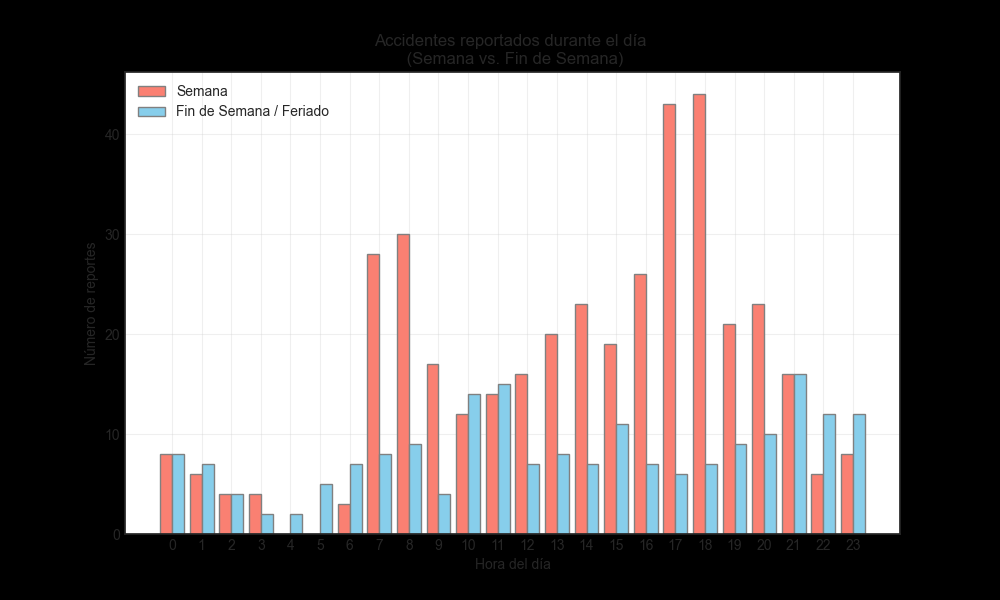
\includegraphics[width=0.6\textwidth]{images/ACCIDENT_per_hour.png}
    }
    \newline
    \subfloat[Congestión]{
        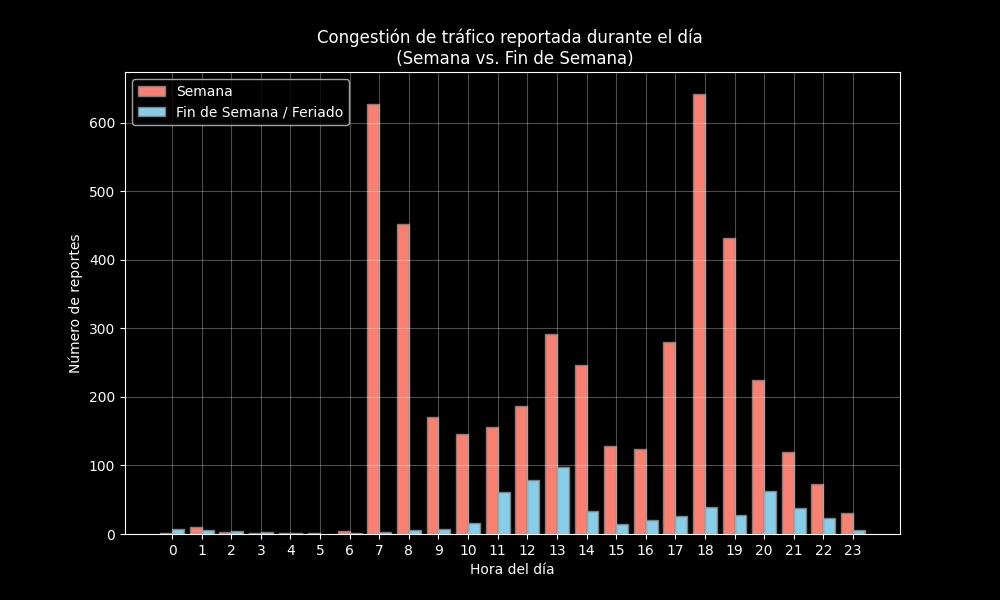
\includegraphics[width=0.6\textwidth]{images/JAM_per_hour.png}
    }
    \newline
    \subfloat[Peligros]{
        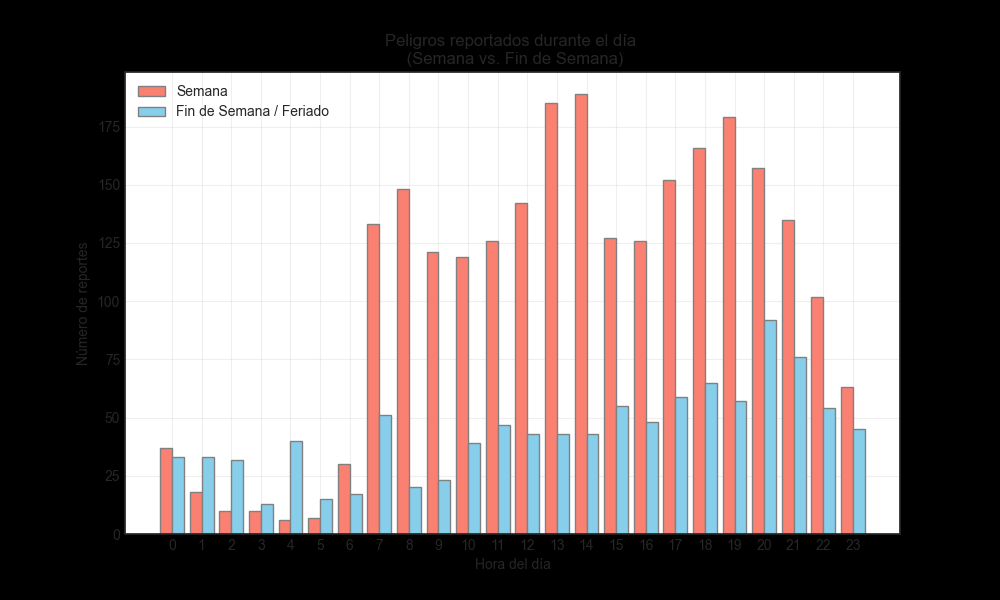
\includegraphics[width=0.6\textwidth]{images/HAZARD_per_hour.png}
    }
    \newline
    \caption{Eventos según hora del día en Antofagasta}
    \label{fig:time_events}
\end{figure}

\subsection{Modelo de correlación lineal}

Los resultados de la regresión lineal entre accidentes y reportes de congestión, presentados en la \cref{fig:corr_lineal}, indican una fuerte correlación positiva durante los días de semana ($R^2 = 0.90$), lo que no implica necesariamente una causalidad. En cambio, durante los fines de semana la relación es más débil ($R^2 = 0.67$), aunque aún presente.

% Prueba hipótesis relación accidents-jams

\begin{figure}[H]
    \centering
    \subfloat[Día de semana]{
        \includegraphics[width=0.9\textwidth]{images/corr_lin_ds.png}
    }
    \newline
    \subfloat[Fin de semana]{
        \includegraphics[width=0.9\textwidth]{images/corr_lin_fs.png}
    }
    \newline
    \caption{Correlación lineal entre accidentes y congestión}
    \label{fig:corr_lineal}
\end{figure}

\subsection{Prueba de hipótesis de correlación lineal}

Para evaluar la existencia de una relación estadísticamente significativa entre el número de reportes de congestión y la cantidad de accidentes por hora, se aplicó una prueba de correlación de Pearson.

La hipótesis nula ($H_0$) establece que no existe correlación lineal entre ambas variables, mientras que la hipótesis alternativa ($H_1$) plantea que sí existe tal correlación:

\begin{align}
H_0&:\ \rho = 0 \\
H_1&:\ \rho \ne 0
\end{align}

Donde $\rho$ representa el coeficiente de correlación poblacional. El estadístico de prueba se calcula mediante:

\begin{equation}
t = \frac{r \sqrt{n - 2}}{\sqrt{1 - r^2}}
\end{equation}

donde $r$ es el coeficiente de correlación muestral y $n$ el número de observaciones. El valor resultante se contrasta con la distribución t de Student con $n - 2$ grados de libertad.

El análisis estadístico del modelo lineal entregó resultados significativos tanto para días de semana como para fin de semana:

\begin{itemize}
    \item Para días de semana:
    \begin{itemize}
        \item El modelo ajustado fue $y = 0.1673x + 0.0996$
        \item Se obtuvo un $R^2 = 0.90$, explicando el 90\% de la variabilidad
        \item La significancia global fue $F(1, 22) = 203.33$, $p < 0.0001$
        \item Los parámetros fueron estadísticamente significativos con $p < 0.001$
        \item El estadístico $t$ para la prueba de correlación fue $t = 14.26$, $p < 0.0001$
    \end{itemize}

    \item Para fines de semana:
    \begin{itemize}
        \item El modelo ajustado fue $y = 0.1365x + 0.0748$
        \item Se obtuvo un $R^2 = 0.67$, explicando el 67\% de la variabilidad
        \item El coeficiente de correlación de Pearson fue $r = 0.82$ con IC 95\%: [0.62, 0.92]
        \item La significancia global fue $F(1, 22) = 44.42$, $p < 0.0001$
        \item Los parámetros fueron estadísticamente significativos con $p < 0.0001$
        \item El estadístico $t$ para la prueba de correlación fue $t = 6.66$, $p < 0.0001$
    \end{itemize}
\end{itemize}

Estos resultados permiten rechazar la hipótesis nula con un nivel de confianza del 99\% para los días de semana, confirmando la existencia de una relación lineal estadísticamente significativa entre el número de reportes de congestión y la cantidad de accidentes registrados por hora.

\begin{figure}[H]
\centering
\includegraphics[width=0.9\textwidth]{images/residuos_lin.png}
\caption{Residuos del modelo lineal para días de semana y fines de semana}
\label{fig:resid_lin}
\end{figure}

\begin{figure}[H]
\centering
\includegraphics[width=0.9\textwidth]{images/qq_lin.png}
\caption{Gráficos Q-Q de los residuos del modelo lineal}
\label{fig:qq_lin}
\end{figure}

Los gráficos Q-Q (\cref{fig:qq_lin}) muestran una aproximación razonable a la distribución normal en ambos períodos. Para los días de semana, los puntos siguen la línea de referencia, con algunas desviaciones en los extremos, particularmente en los valores más altos. En el caso de fin de semana, la aproximación a la línea teórica es más consistente, con una distribución más cercana a la normal.

Los gráficos de residuos (\cref{fig:resid_lin}) revelan patrones distintos para cada período. En días de semana, aunque hay cierta dispersión alrededor de cero, se observa variabilidad considerable con algunos residuos positivos destacados (especialmente entre valores ajustados de 0.5 y 0.6) y residuos negativos pronunciados alrededor de 0.8. Para fines de semana, los residuos muestran menor magnitud global, pero un patrón menos aleatorio, sugiriendo posible estructura no capturada por el modelo lineal.

En resumen, el análisis confirma una relación lineal significativa entre congestión y accidentes, considerablemente más fuerte durante días laborables ($R^2 = 0.90$) que en fines de semana ($R^2 = 0.67$). Los patrones observados en los residuos, particularmente para fines de semana, sugieren la pertinencia de explorar modelos no lineales que podrían capturar mejor las relaciones subyacentes en los datos.


\subsection{Modelo de correlación exponencial inversa}

Dado que la relación entre congestión y accidentes no necesariamente es lineal en todos los contextos —especialmente bajo alta densidad vehicular— se propuso un modelo exponencial inverso.

El modelo propuesto se ajusta a la siguiente forma funcional:

\begin{equation}
A(x) = \frac{\alpha}{x^{\beta}} + \gamma
\end{equation}

donde:
\begin{itemize}
    \item $A(x)$ es el número estimado de accidentes por hora,
    \item $x$ representa el número de reportes de congestión por hora,
    \item $\alpha$, $\beta$ y $\gamma$ son parámetros ajustados mediante regresión no lineal.
\end{itemize}

Este modelo fue aplicado tanto a los días de semana como a los fines de semana. En ambos casos, se observó un ajuste visual considerable, respaldando la hipótesis de una relación decreciente no lineal entre ambas variables bajo ciertas condiciones de tráfico.

Los resultados del ajuste se presentan en la \cref{fig:corr_exp}, mostrando un ajuste significativo del modelo a los datos.

\begin{figure}[H]
    \centering
    \subfloat[Día de semana]{
        \includegraphics[width=0.9\textwidth]{images/corr_exp_ds.png}
    }
    \newline
    \subfloat[Fin de semana]{
        \includegraphics[width=0.9\textwidth]{images/corr_exp_fs.png}
    }
    \newline
    \caption{Correlación exponencial inversa entre accidentes y congestión}
    \label{fig:corr_exp}
\end{figure}

El análisis estadístico del modelo exponencial inverso entregó resultados significativos tanto para días de semana como para fin de semana:

\begin{itemize}
    \item Para días de semana:
    \begin{itemize}
        \item El modelo ajustado fue $y = 0.3119/x^{-0.6319}$
        \item Se obtuvo un $R^2 = 0.94$, explicando el 94\% de la variabilidad
        \item La significancia global fue $F(2, 22) = 158.81$, $p < 0.0001$
        \item Los parámetros fueron estadísticamente significativos con $p < 0.0001$
    \end{itemize}

    \item Para fines de semana:
    \begin{itemize}
        \item El modelo ajustado fue $y = 0.1826/x^{-0.2776}$
        \item Se obtuvo un $R^2 = 0.71$, explicando el 71\% de la variabilidad
        \item La significancia global fue $F(2, 22) = 27.19$, $p < 0.001$
        \item Los parámetros fueron estadísticamente significativos con $p < 0.001$
    \end{itemize}
\end{itemize}

Este análisis revela diferencias importantes en la dinámica de la relación congestión-accidentes entre períodos. Durante los días de semana, el exponente negativo de mayor magnitud ($-0.6319$) indica una relación más sensible entre las variables, mientras que en fines de semana el exponente menor ($-0.2776$) sugiere una relación menos pronunciada.

\begin{figure}[H]
\centering
\includegraphics[width=0.9\textwidth]{images/residuos_exp.png}
\caption{Residuos del modelo de exponencial inverso para días de semana y fines de semana}
\label{fig:resid_exp}
\end{figure}

\begin{figure}[H]
\centering
\includegraphics[width=0.9\textwidth]{images/qq_exp.png}
\caption{Gráficos Q-Q de los residuos del modelo exponencial inverso}
\label{fig:qq_exp}
\end{figure}

Los gráficos de residuos (\cref{fig:resid_exp}) muestran una dispersión relativamente aleatoria en torno a cero, sin evidencias claras de heterocedasticidad ni patrones sistemáticos, lo que respalda la validez del ajuste no lineal propuesto. En particular, para los días de semana, los residuos muestran una distribución uniforme con algunos valores extremos (entre -0.1 y 0.2), mientras que para los fines de semana, la dispersión es menor y más equilibrada (aproximadamente entre -0.05 y 0.05).

Complementariamente, los gráficos Q-Q (\cref{fig:qq_exp}) revelan una aproximación a la distribución normal de los residuos en ambos casos, aunque con algunas desviaciones. En días de semana, se observan algunas desviaciones en los valores extremos, particularmente un punto notable en el extremo positivo. Para los fines de semana, la alineación con la línea teórica es excepcional, indicando una distribución muy cercana a la normal.

En conjunto, estos resultados indican que el modelo exponencial inverso no solo es estadísticamente significativo, sino que además presenta un mejor ajuste que el modelo lineal, especialmente para días de semana donde alcanza un $R^2 = 0.94$ comparado con el $R^2 = 0.90$ del modelo lineal. La normalidad de los residuos y su distribución aleatoria fortalecen la hipótesis de que existe una relación no lineal entre la congestión y la probabilidad de accidentes en contextos urbanos, que puede ser modelada adecuadamente mediante una función exponencial inversa.

% Cálculo de la frecuencia por zona
% Filtro por zona
%    Algóritmo cKDTree

\subsection{Frecuencia por zona} \label{ssec:freq_zone}

Para representar conjuntos estáticos de puntos espaciales, se utiliza la estructura Kd-tree que computa distancias relativas mediante spiral codes y las almacena usando Directly Addressable Codes (DACs), optimizando el uso de memoria sin sacrificar eficiencia en consultas espaciales \citep{gutierrez2023ckdtree}. Cada zona es llamada cuadrante o segmento.

En la \cref{fig:quad_acc} se puede ver cómo se distribuyen los segmentos numéricamente, comenzando desde el segmento 1 en la esquina inferior izquierda. La opacidad del color rojo está relacionada con la cantidad de accidentes por segmento.

\begin{figure}[H]
    \centering
    \includegraphics[width=0.38\textwidth]{images/quad_acc.png}
    \caption{Identificación de cuadrantes en mapa de Antofagasta}
    \label{fig:quad_acc}
\end{figure}

Considerando la media de accidentes diarios, se agrupa por segmento, se define que las zonas mayores a 0.5 accidentes por día son considerados críticos, se construye un mapa según la criticidad (\cref{fig:quad_mean_day}), al tomar la suma de los accidentes, se obtiene la \cref{fig:quad_acc_total} que muestra la cantidad de accidentes reportados en el segmento en el periodo de estudio, que a su vez se clasifican como críticos si poseen más de 90 accidentes.


\begin{figure}[H]
    \centering
    \subfloat[Media de accidentes por día]{
        \includegraphics[width=0.4\textwidth]{images/quad_mean_day_color.png}
        \label{fig:quad_mean_day}
    }
    \subfloat[Total accidentes]{
        \includegraphics[width=0.4\textwidth]{images/quad_acc_color.png}
        \label{fig:quad_acc_total}
    }
    \caption{Accidentes por segmento}
\end{figure}


% Ruta más segura

% Machine learning (XGBoost)

\subsection{Selección del modelo de Machine Learning}

Se evaluaron distintos algoritmos de clasificación para abordar el problema planteado. Inicialmente, se probaron modelos clásicos como \textit{Logistic Regression}, \textit{K-Nearest Neighbors}, \textit{Decision Tree}, entre otros. Sin embargo, estos no mostraron mejoras relevantes en las métricas evaluadas, por lo que se descartaron para la fase de ajuste de hiperparámetros.

Se procedió entonces a aplicar una búsqueda exhaustiva (\textit{GridSearchCV}) sobre dos modelos con buen desempeño preliminar: \textbf{Random Forest} y \textbf{XGBoost}.

\paragraph{Random Forest}
Se evaluaron los siguientes hiperparámetros:

\begin{itemize}
    \item \texttt{max\_depth}: [2, 5, 10]
    \item \texttt{n\_estimators}: [20, 80, 100, 200]
    \item \texttt{min\_samples\_leaf}: [2, 4, 8]
    \item \texttt{max\_leaf\_nodes}: [2, 8]
    \item \texttt{max\_features}: [2, 8]
    \item \texttt{class\_weight}: [None, 'balanced']
\end{itemize}

Los mejores hiperparámetros obtenidos fueron:

\begin{itemize}
    \item \texttt{class\_weight}: None
    \item \texttt{max\_depth}: 10
    \item \texttt{max\_features}: 2
    \item \texttt{max\_leaf\_nodes}: 8
    \item \texttt{min\_samples\_leaf}: 2
    \item \texttt{n\_estimators}: 100
\end{itemize}

Con estos valores, el modelo alcanzó una puntuación máxima de \textbf{0.7957} en validación cruzada.


\paragraph{XGBoost.}
Se aplicaron múltiples rondas de \textit{grid search} con distintos rangos de hiperparámetros, refinando progresivamente los valores. Los mejores resultados se obtuvieron con:

\begin{itemize}
    \item \texttt{colsample\_bytree}: 0.7
    \item \texttt{gamma}: 1
    \item \texttt{learning\_rate}: 0.1
    \item \texttt{max\_depth}: 30
    \item \texttt{n\_estimators}: 80
\end{itemize}

Este modelo logró una métrica de validación cruzada de \textbf{0.8665}, superando significativamente al resto de las alternativas evaluadas. Por este motivo, \textbf{XGBoost fue seleccionado como modelo final}.

En el \cref{tab:model-comparison} se puede observar la comparación de ambos modelos.

\begin{table}[H]
\centering
\begin{tabular}{|l|p{9cm}|c|}
\hline
\textbf{Modelo} & \textbf{Mejores Hiperparámetros} & \textbf{Mejor Score} \\
\hline
\textbf{Random Forest} &
\begin{tabular}[c]{@{}l@{}}
\texttt{class\_weight}: None\\
\texttt{max\_depth}: 10\\
\texttt{max\_features}: 2\\
\texttt{max\_leaf\_nodes}: 8\\
\texttt{min\_samples\_leaf}: 2\\
\texttt{n\_estimators}: 100
\end{tabular}
& 0.7957 \\
\hline
\textbf{XGBoost} &
\begin{tabular}[c]{@{}l@{}}
\texttt{colsample\_bytree}: 0.7\\
\texttt{gamma}: 1\\
\texttt{learning\_rate}: 0.1\\
\texttt{max\_depth}: 30\\
\texttt{n\_estimators}: 80
\end{tabular}
& \textbf{0.8665} \\
\hline
\end{tabular}
\caption{Comparativa de modelos ajustados con GridSearchCV}
\label{tab:model-comparison}
\end{table}


\subsection{Generación de eventos negativos simulados} \label{ssec:class_balancing}

Dado que el conjunto original contiene únicamente eventos positivos (ocurridos), fue necesario generar instancias negativas (no ocurridos) para entrenar un modelo de clasificación binaria. Para ello, se implementó una estrategia inspirada en el enfoque de generación de eventos negativos artificiales propuesto por Goedertier et al. \citep{goedertier2009robust}, que permite representar problemas secuenciales como tareas de clasificación supervisada.

En este caso, la generación se basa en una grilla temporal con intervalos de 5 minutos, sobre la cual se combinan todas las posibles ubicaciones (\texttt{segmento}) y tipos de evento. Se identifican aquellas combinaciones que no se encuentran en los datos originales —donde no ocurrió un evento— y se etiquetan como eventos negativos (\texttt{happen} = 0). Estas instancias se muestrean de forma aleatoria para igualar la cantidad de eventos positivos, logrando así un conjunto balanceado con un 50\% de eventos positivos y 50\% de negativos.

Este enfoque permite mantener la estructura temporal y geoespacial de los datos reales, evitando introducir ruido aleatorio, y facilitando la evaluación robusta de métricas como \texttt{recall} y \texttt{precision}.


\subsection{Resultados del modelo seleccionado}

La versión final del modelo (\texttt{v6}) se entrenó utilizando los hiperparámetros obtenidos durante la etapa de validación cruzada. El modelo fue registrado y versionado mediante \textit{MLflow}, permitiendo un seguimiento detallado de sus parámetros y métricas.

El modelo utiliza codificación \textit{one-hot} y un esquema de clasificación binaria (\texttt{binary:logistic}), con una semilla aleatoria (\texttt{random\_state = 42}) para garantizar la reproducibilidad \citep{geron2019hands}


\noindent En cuanto al rendimiento, se obtuvieron los siguientes resultados para una muestra de 64.708 eventos, con un 50\% de eventos ocurridos y un 50\% de no ocurridos. Esta proporción se logró mediante la simulación de eventos negativos sobre una grilla temporal de 5 minutos, generando combinaciones posibles de tiempo, localización y tipo de evento que no están presentes en los datos originales (\cref{ssec:class_balancing}). Esto permite evaluar el modelo en condiciones balanceadas, facilitando la interpretación de métricas como \texttt{precision}, \texttt{recall} y \texttt{F1-score}.

\begin{itemize}
    \item \textbf{Accuracy}: 0.8795
    \item \textbf{Recall}: 0.9076
    \item \textbf{Precision}: 0.8583
    \item \textbf{F1-score}: 0.8823
    \item \textbf{Promedio validación cruzada (10 folds)}: 0.7819
\end{itemize}

\noindent Respecto a la matriz de confusión, se registraron los siguientes valores:

\begin{itemize}
    \item Verdaderos positivos: 5,539
    \item Verdaderos negativos: 5,843
    \item Falsos positivos: 965
    \item Falsos negativos: 595
\end{itemize}

Estas métricas evidencian un modelo con gran capacidad para identificar correctamente los casos positivos, sin sacrificar precisión ni equilibrio. La validación cruzada muestra estabilidad a lo largo de los distintos \texttt{folds}, lo que refuerza la robustez del modelo final y confirma que no hubo sobreentrenamiento \citep{geron2019hands}.

\subsection{Curva de aprendizaje del modelo}

La \cref{fig:learning_curve} muestra la curva de aprendizaje del modelo XGBoost entrenado. Se observa un rendimiento alto y consistente tanto en el conjunto de entrenamiento como en el de validación (aproximadamente 0.88–0.90), con una brecha mínima entre ambas curvas. Esto indica que el modelo generaliza adecuadamente, sin presentar sobreajuste ni subajuste. Además, el comportamiento plano de ambas curvas sugiere que incrementar el tamaño del conjunto de entrenamiento no tendría un impacto significativo en el rendimiento, lo cual evidencia una saturación en la capacidad de aprendizaje del modelo con las características actuales.


\begin{figure}[H]
    \centering
    \includegraphics[width=0.8\textwidth]{images/learning_curve.png}
    \caption{Identificación de cuadrantes en mapa de Antofagasta}
    \label{fig:learning_curve}
\end{figure}

% Aplicación implementacióñ (dashboard online y ML)

\subsection{Despliegue y mantenimiento del modelo}

Para entregar una interfaz que permita al usuario final interactuar con los datos, se desarrolló un tablero de control utilizando \texttt{Dash}, un marco de trabajo especializado en la presentación de datos gráficos mediante Python. La arquitectura del sistema se diseñó siguiendo el patrón cliente-servidor: el servidor implementado en Rust y el cliente en Python, como se muestra en la \cref{fig:architecture}. El servidor se encarga de las operaciones intensivas como la captura, transformación, almacenamiento y gestión del caché de los datos, mientras que el cliente maneja la interacción con el usuario, la actualización de datos desde el servidor, el entrenamiento del modelo y la generación del tablero de control.

El ciclo de vida del modelo se gestiona mediante APScheduler. Esto permite automatizar el re-entrenamiento periódico del modelo con nuevos datos, garantizando su actualización y adaptación a los cambios en los patrones de tráfico. El proceso incluye la validación automática del rendimiento del modelo, comparando las métricas clave (precisión, recall, F1-score) con los umbrales establecidos, y solo se despliega una nueva versión si representa una mejora en el F1-score.

En el servidor se utiliza Memcached como sistema de caché para optimizar el acceso a los datos frecuentemente consultados, implementando una estrategia de almacenamiento que prioriza la unicidad de los datos para minimizar el uso de memoria. En el lado del cliente, se implementa un sistema de workers múltiples que comparten una única instancia de los datos en memoria, protegida mediante un \texttt{Mutex} para garantizar la integridad en las operaciones de lectura concurrentes.

\begin{figure}[H]
    \centering
    \includegraphics[width=0.8\textwidth]{images/dashboard.png}
    \caption{Arquitectura del sistema}
    \label{fig:architecture}
\end{figure}

El entrenamiento del modelo está programado para realizarse cada 30 días, utilizando los nuevos datos. Los datos del dashboard se actualizan cada 5 minutos.


\section{Discusiones}

Los análisis espaciales y temporales realizados permitieron identificar patrones críticos en la ocurrencia de accidentes en Antofagasta. En la \cref{fig:quad_acc_total} se observan las zonas con mayor concentración de accidentes, destacando los segmentos ubicados en el eje de la avenida Pedro Aguirre Cerda, especialmente en el cruce con Nicolás Tirado (segmentos 106 a 109). Este corredor vial presenta una densidad particularmente alta, lo que lo posiciona como un foco de atención prioritaria.

Se identificó un segundo punto crítico en la intersección entre la Avenida Salvador Allende y Edmundo Pérez Zujovic, donde convergen flujos de alto volumen provenientes del norte y del centro de la ciudad. Esta área (segmentos 84 y 103) también mostró una alta frecuencia de accidentes diarios, como se observa en la \cref{fig:quad_mean_day}.

El centro de la ciudad, particularmente en segmento 82, evidenció una densidad considerable de accidentes.

Los modelos estadísticos desarrollados mostraron una fuerte correlación entre congestión y accidentes, especialmente durante los días de semana. El modelo de potencia inversa entregó un mejor ajuste ($R^2 = 0.96$) que el modelo lineal ($R^2 = 0.92$), capturando de mejor forma la dinámica decreciente del riesgo bajo alta congestión.

Finalmente, el modelo predictivo XGBoost alcanzó un desempeño sobresaliente (\textbf{F1-score = 0.8823}, \textbf{Recall = 0.9076}), confirmando su utilidad como herramienta predictiva y de soporte en la toma de decisiones en gestión vial.

% Observaciones y resultados del estudio

% \section{Discusión}

% Preguntas y posibles soluciones

\section{Conclusiones}

Este estudio demuestra la factibilidad y el impacto del uso de datos colaborativos para la gestión inteligente del tráfico urbano. A través de una arquitectura eficiente y una metodología robusta, se logró:

\begin{itemize}
    \item Identificar zonas críticas con alta concentración de accidentes, como el cruce de Nicolás Tirado con Pedro Aguirre Cerda, la intersección de Salvador Allende con Edmundo Pérez Zujovic, y sectores del centro de Antofagasta.
    \item Confirmar la existencia de una relación estadísticamente significativa entre los reportes de congestión y los accidentes, siendo más fuerte durante los días de semana.
    \item Validar el uso de modelos no lineales como herramientas más adecuadas para representar fenómenos de tráfico en contextos urbanos densos.
    \item Desarrollar un modelo predictivo basado en XGBoost con alto rendimiento, capaz de anticipar la ocurrencia de accidentes con gran precisión.
    \item Implementar un sistema funcional de monitoreo y visualización que permite actualizar el modelo periódicamente y ofrecer datos en tiempo real a los usuarios finales.
\end{itemize}

Se concluye que el enfoque propuesto no solo es viable, sino escalable, y representa una base sólida para iniciativas de movilidad urbana basadas en datos.

\section{Recomendaciones}

A partir de los resultados obtenidos, se proponen las siguientes recomendaciones para autoridades locales, planificadores urbanos y futuras investigaciones:

\begin{itemize}
    \item \textbf{Intervención en zonas críticas}: Priorizar acciones de ingeniería vial, señalización y fiscalización en los segmentos identificados como críticos, particularmente en el eje Pedro Aguirre Cerda, Salvador Allende y el centro de la ciudad.
    \item \textbf{Monitoreo continuo}: Mantener y escalar el sistema de recolección y análisis de datos, integrando nuevas fuentes (sensores, cámaras) para enriquecer el modelo.
    \item \textbf{Validación en terreno}: Complementar los hallazgos con estudios de campo para confirmar condiciones geométricas, flujos vehiculares y comportamiento de los usuarios en las zonas críticas.
    \item \textbf{Extensión del sistema}: Replicar esta metodología en otras ciudades de tamaño medio que carezcan de infraestructura de monitoreo formal \citep{berhanu2024}.
    \item \textbf{Nuevas líneas de investigación}: Incorporar variables climáticas, de infraestructura o comportamiento humano para enriquecer los modelos predictivos y explorar algoritmos más avanzados (LSTM, transformers, modelos causales).
\end{itemize}

Estas recomendaciones apuntan a fortalecer una gestión vial basada en datos, proactiva y centrada en la seguridad de los ciudadanos.

\newpage

\appendix
\section{Transformación de coordenadas UTM}
\label{ap:utm}

La proyección UTM utilizada en este estudio (EPSG:32719) se basa en la proyección Transversa de Mercator, adaptada al hemisferio sur y centrada en el meridiano $\lambda_0 = -69^\circ$. Esta proyección es conforme y está diseñada para minimizar la distorsión métrica en una zona longitudinal específica (zona 19S), siendo especialmente adecuada para representar regiones como Antofagasta.

A continuación se presentan las fórmulas que permiten convertir coordenadas geográficas $(\phi, \lambda)$ —latitud y longitud en radianes— a coordenadas planas proyectadas $(x, y)$ en metros, basadas en el elipsoide WGS84:

\subsection*{Parámetros del elipsoide WGS84}

\begin{itemize}
  \item Semieje mayor: $a = 6378137.0$ m
  \item Aplanamiento: $f = \frac{1}{298.257223563}$
  \item Excentricidad: $e^2 = 2f - f^2$
  \item Factor de escala: $k_0 = 0.9996$
  \item Falso este: $E_0 = 500\,000$ m
  \item Falso norte (hemisferio sur): $N_0 = 10\,000\,000$ m
\end{itemize}

\subsection*{Variables intermedias}

\begin{align*}
e'^2 &= \frac{e^2}{1 - e^2} \\
N &= \frac{a}{\sqrt{1 - e^2 \sin^2 \phi}} \\
T &= \tan^2 \phi \\
C &= e'^2 \cos^2 \phi \\
A &= (\lambda - \lambda_0) \cos \phi
\end{align*}

\subsection*{Cálculo del arco meridiano}

\begin{align*}
M &= a \cdot \left[
(1 - \frac{e^2}{4} - \frac{3e^4}{64} - \frac{5e^6}{256}) \phi \right. \\
&\quad - (\frac{3e^2}{8} + \frac{3e^4}{32} + \frac{45e^6}{1024}) \sin(2\phi) \\
&\quad + (\frac{15e^4}{256} + \frac{45e^6}{1024}) \sin(4\phi) \\
&\quad \left. - (\frac{35e^6}{3072}) \sin(6\phi)
\right]
\end{align*}

\subsection*{Coordenadas proyectadas}

\begin{align*}
x &= E_0 + k_0 N \left[ A + \frac{A^3}{6}(1 - T + C) + \frac{A^5}{120}(5 - 18T + T^2 + 72C - 58e'^2) \right] \\
y &= N_0 + k_0 \left[ M + N \tan \phi \left( \frac{A^2}{2} + \frac{A^4}{24}(5 - T + 9C + 4C^2) + \frac{A^6}{720}(61 - 58T + T^2 + 600C - 330e'^2) \right) \right]
\end{align*}

Estas expresiones corresponden a un desarrollo en serie basado en una expansión de Taylor, que permite una transformación precisa desde la superficie curva del elipsoide a un plano cartesiano. Estas fórmulas son utilizadas internamente por la biblioteca PROJ, y fueron documentadas formalmente por Snyder \citep{snyder_tm}.

\subsection*{Nota}

La implementación computacional de estas fórmulas puede realizarse utilizando bibliotecas como \texttt{Pyproj}, que encapsulan estos desarrollos y gestionan automáticamente los parámetros de cada sistema de referencia (CRS).


\newpage


\bibliography{biblio}
\end{document}

